\section{Business Process-Dokumentation}

\subsection{Prozessübersicht}

Im Projekt wurden drei zentrale Geschäftsprozesse abgebildet: die Registrierung, die Authentifizierung (Login) und die Reisesuche mit optionaler Speicherung.

Bei der Registrierung werden Benutzerdaten wie E-Mail, Passwort und Name über das Frontend erfasst und an den Authentication-Microservice übergeben. Dort erfolgt mithilfe der Bibliothek Pydantic v2 eine Datenvalidierung, wodurch Eingabefehler frühzeitig erkannt werden. Das Passwort wird mit dem sicheren Hashing-Verfahren bcrypt verschlüsselt und anschließend in einer PostgreSQL-Datenbank gespeichert.

Beim Login wird der Nutzer erneut über E-Mail und Passwort authentifiziert. Bei erfolgreicher Anmeldung wird ein sogenannter JWT-Token (JSON Web Token) erstellt und dem Nutzer übermittelt. Dieser Token dient als Identitätsnachweis und wird bei nachfolgenden Anfragen an andere Microservices verwendet, um den Nutzer zu identifizieren.

Ein weiterer zentraler Prozess ist die Reisesuche. Nach erfolgreicher Authentifizierung kann der Nutzer über das Frontend individuelle Wünsche und Kriterien für seine Reise eingeben. Diese Informationen werden an den Travel-Planner-Microservice übergeben. Dieser analysiert die Daten mithilfe des Sprachmodells Gemini und generiert daraufhin passende Reisezielvorschläge. Die Ergebnisse werden im Frontend ausgegeben. Nutzer haben anschließend die Möglichkeit, eine Reise dauerhaft zu speichern. Dabei wird mithilfe des JWT-Tokens überprüft, ob der Nutzer angemeldet ist. Die Reiseinformationen werden dann in einer MongoDB-Datenbank abgelegt und mit einer eindeutigen Nutzerkennung verknüpft. Auf diese Weise ist sichergestellt, dass jeder Nutzer nur Zugriff auf seine eigenen gespeicherten Reisen hat.

Zur Umsetzung dieser Prozesse wurden gezielt technische Maßnahmen gewählt, die die Anforderungen des Systems effektiv unterstützen. Die Nutzung von FastAPI als Framework ermöglicht eine schnelle und effiziente Entwicklung der REST-Schnittstellen. Durch die Integration von Swagger UI kann die API direkt getestet werden, was insbesondere während der Entwicklung und im Austausch mit anderen Projektteilen von Vorteil ist. Die Kombination aus JWT-basiertem Login, bcrypt zur Passwortverschlüsselung sowie einer klaren Trennung zwischen Authentifizierung und Anwendungslogik über Microservices trägt zur Sicherheit und Skalierbarkeit des Systems bei. Die Datenvalidierung über Pydantic sorgt für Robustheit und reduziert Fehlerquellen bereits bei der Eingabe.

\subsection{User-Gruppen}

Grundsätzlich gibt es zwei User-Gruppen, die in der Business Process-Dokumentation berücksichtigt werden müssen:

\begin{itemize}
    \item \textbf{End-User}: Diese Gruppe umfasst alle Personen, die das System nutzen, um sich Reisen empfehlen zu lassen und auf ihrem Profil zu speichern.
    \item \textbf{Administratoren}: Diese Gruppe sitzt hinter dem System und kann Einsichten in analytiscshe Informationen des Systems gewinnen.
\end{itemize}

\subsubsection{Prozesse für End-User}

Ein End-User kann folgende Prozesse durchlaufen:

\begin{itemize}
    \item \textbf{Registrierung}: Der End-User registriert sich im System, um ein Nutzerprofil zu erstellen. Dabei gibt er seinen Namen, E-Mail-Adresse und Passwort an. Diese Informationen werden über den Authentifizierungsservice verarbeitet und in der Datenbank gespeichert.
    \item \textbf{Login}: Der End-User meldet sich an, um auf sein Profil und die Reiseempfehlungen zuzugreifen. Hierbei werden die Anmeldedaten überprüft und ein JWT-Token generiert, der für die Authentifizierung bei weiteren Anfragen verwendet wird.
    \item \textbf{Reiseempfehlung anfordern}: Der End-User kann eine Anfrage für personalisierte Reiseempfehlungen stellen. Hierbei kann er verschiedene Parameter wie Reisedauer oder Budget angeben. Die Anfrage wird hier etwas "gemockt". Die Logik für die Empfehlungen wurde wegen dem großen Umfang nicht implementiert. Die Konfiguration wird einfach an eine API von Google GenAI weitergeleitet, die dann eine Antwort zurückgibt.
    \item \textbf{Reise speichern}: Der End-User kann empfohlene Reisen in seinem Profil speichern. Hierzu ist eine OAuth2-Authentifizierung mit dem Authentifizierungsservice erforderlich. Die gespeicherten Reisen werden in einer NoSQl-Datenbank gespeichert, versehen mit der Information, welchem Nutzer sie zugeordnet sind.
    \item \textbf{Reisen anzeigen}: Der End-User kann seine gespeicherten Reisen einsehen. Die Daten werden aus der NoSQL-Datenbank abgerufen und im Frontend angezeigt.
\end{itemize}

\subsubsection{Prozesse für Administratoren}

Für den Administrator gibt es nur einen Prozess:

Es gibt ein sehr einfaches Dashboard ohne jegliche Authentifizierung, das bloß dazu dient, zwei Tabellen aus den gespeicherten Log-Daten anzuzeigen. Die Tabellen enthalten die meist-gesuchten Reiseziele und die beliebtesten Ortsarten (z.B. Strand, Berge, Stadt). Diese Daten werden aus der NoSQL-Datenbank abgerufen und im Frontend angezeigt. Der Administrator kann so einen Überblick über die Nutzung des Systems gewinnen.

\begin{figure}[h]
    \centering
    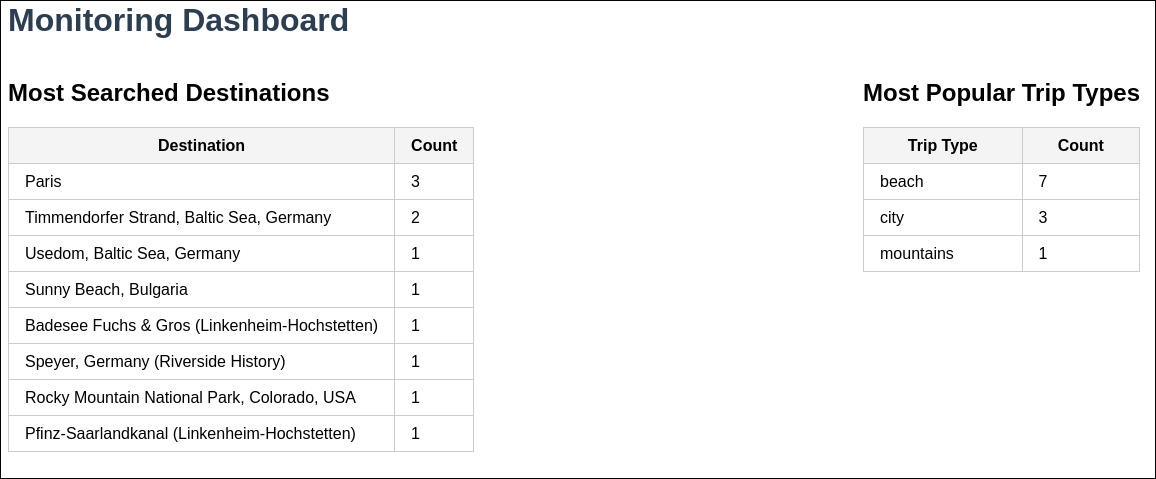
\includegraphics[width=0.8\textwidth]{images/monitoring.png}
    \caption{Monitoring-Dashboard}
\end{figure}

\subsection{Schritt-für-Schritt-Durchlauf}

Startet man die Anwendung das Erste Mal, sieht man eine Login-Seite. Hier kann man sich mit der angegebenen E-Mail-Adresse und dem Passwort anmelden, sofern man einen Account hat. Hat man noch keinen Account erstellt, kann man dies über den Knopf \enquote{Register now} machen.

Auf der Register-Seite kann man mit E-Mail-Adresse, Name und Passwort einen Account erstellen. Gibt man zulässige Daten an und klickt auf \enquote{Register}, wird man zu einer \enquote{Success}-Seite weitergeleitet, die die erfolgreiche Registrierung bestätigt.
Hier kann man dann wieder zurück zur Login-Seite und sich mit den neu erstellten Accountdaten anmelden.

Nach dem erfolgreichen Login gelangt man zu einer persönlichen Startseite, auf welcher gespeicherte Reisen angezeigt werden. Will man eine neue Reise planen, geht dies über den Button \enquote{Plan a Trip}.

Um dann Reiseempfehlungen zu erhalten, muss man zunächst einige Angaben machen. Hierbei müsen \enquote{Recidency, Maximum Cost, Duration, Destination Type und Preferred Temperature} angegeben werden.

Durch den Klick auf den Button \enquote{Get Recommendations} wird eine Anfrage an die Google GenAI API geschickt, die diese Angaben beinhaltet. Die API gibt dann eine Liste von fünf Reiseempfehlungen zurück. Auf der Übersichtseite werden diese mit einer Kurzbeschreibung angezeigt. Über den Button \enquote{Details} gelangt man zu einem detaillierten Reiseplan, der Empfehlungen für jeden Tag der Reise sowie allgemeine Reisetipps enthält. Unten auf der Seite, kann man die Reise speichern, um sie später wieder anschauen zu können. Beim Speichern wird man wieder auf die persönliche Startseite weitergeleitet, wo alle gespeicherten Reisen angezeigt werden.
Über den Button \enquote{View Details} kann man auch die Details der gespeicherten Reisen einsehen.

Über die Home-Schaltfläche oben links gelangt man jederzeit zurück zur persönlichen Startseite. Klickt man oben rechts auf \enquote{Account}, kann man den Username und Full Name einsehen, sowie sich ausloggen. Loggt man sich aus, wird man wieder auf die Login-Seite weitergeleitet.
 
